\chapter{Sensor Application}\label{sensor-application}
In this chapter the sensor application will be presented. 
Several sequence diagrams will be explained, as well as concepts needed to understand the flow of the application. 

\section{Health Sensors}
There is an ongoing discussion of when the health technology revolution will come to human bodies now that \gls{IoT} have become so popular.
By revolution, I mean sensors placed in the human body. 
Sensors that can read your blood pressure, heart rate and measure insulin levels.
Sensors that can detect whether your body is missing a substance, or if it is poisoned. 
There is no limit for what can be done.
Everything that should be measured, will be measured by sensors integrated in the human body.
But who will be able to read the \gls{data}?
Or perform instructions to the sensors/devices?
There is some major privacy issues related to this discussion, and problems that needs to be solved.

In 2011, Jerome Radcliffe discovered that his insulin pump easily could be hacked~\cite{radcliffe2011hacking}.
Basically the pump would take instructions from anyone and do anything, with no questions asked. 
This is a worst case scenario when it comes to hacking medical devices attached to a human.

For this matter I propose a \gls{HSS} that is built upon \gls{NDN} with \gls{IBC} ensuring a secure and locked environment.
First, let me introduce you to The Stig. 
He has developed diabetes and he does not want to manually monitor his glucose levels and adjust the insulin pump every meal. 
He has injected a \gls{CGM} to monitor his glucose levels and report to the insulin pump, automatically.
In addition to his diabetes, he has a heart disease which forces him to monitor his heart rate at any given time. 
In~\autoref{fig:health-sensor-system} we can see The Stig with all his sensors and devices. 
The \gls{CGM} reports periodically to the insulin pump, and all sensors reports to The Stig's mobile so that The Stig can watch what is going on.

\begin{figure}[ht]
  \centering
  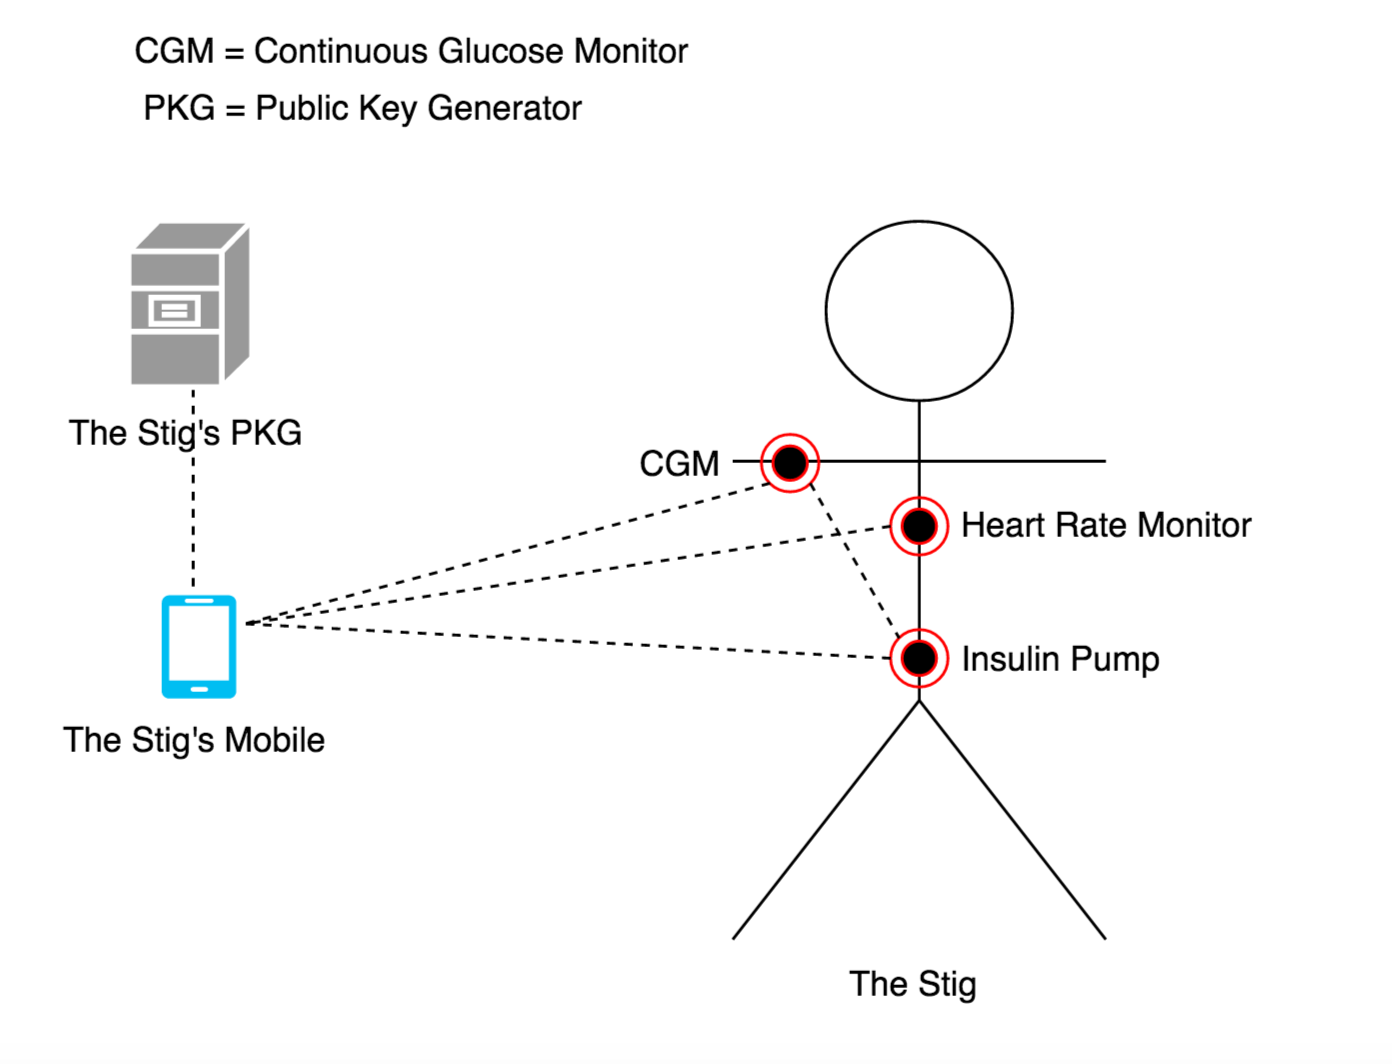
\includegraphics[width=1\textwidth]{health-sensor-system.png}
  \caption{Health Sensor System}
  \label{fig:health-sensor-system}
\end{figure}

\section{Health Sensor System}\label{hss}
To have a secure system, it needs to be established trust between the sensors and the devices.
There need to be integrity controls, confidentiality protection and access control. 
In the following sections, I will describe the protocols suggested for achieving the mentioned goals.

\subsection{Rendezvous Authentication}\label{rendezvous_authentication}
One of the best solutions for authentication of an identity in cryptography is rendezvous authentication, the concept of meeting face-to-face for authenticating who you are talking to. 
Most cases in \gls{IoT} we have the advantage of identifying devices in a physical manner.
This means that it is possible to authenticate devices, such as sensors. 
Typically, this kind of authentication will rely on 1) manually inspection and 2) digital connection, e.g. through \gls{NFC}.
In the proposed system, I assume that this type of authentication is achieved in a secure manner and do not discuss how this should be done.

Also there is the concept of human-computer authentication~\cite{DBLP:journals/iacr/GilbertRS05, DBLP:conf/crypto/JuelsW05, DBLP:conf/percom/Weis05}.
This authentication method uses a shared secret before authentication. 

\subsection{System Initialization Phase}
\todo{refactor section}
When The Stig is setting up his \gls{HSS}, first he wants to configure the \gls{PKG}. 
Any type of computer can play the role of the \gls{PKG} and The Stig has chosen his home server, from now ``the PKG''.
The \gls{PKG} runs the \texttt{Setup()} which creates key pairs that is used to do \gls{IBE} and \gls{IBS}.
Second, he wants his mobile device, from now ``the mobile'', to be a part of the \gls{PKG}s trust domain, and further add all of the other devices and sensors, from now ``device(s)''.

\subsection{Device Registration Phase}\label{init}
The goal for the device registration protocol is to achieve a secure one-round secret key exchange.
For the protocol to be secure, there are several issues that need to be addressed. 
1) The response message containing the secret key has to be encrypted. 
This can be achieved by using a pre-shared symmetric key to do encryption on the \gls{SK}.
2) The response message has to be signed by the \gls{PKG} for integrity and authenticity reasons.
3) A nonce have to be present for replay protection.
The pre-shared symmetric key should be a temporary random generated key. 
Thus the device registration \gls{interest} between the device and the \gls{PKG} can be unique.
This implies that the device can authenticate itself in a way that an adversary cannot do.

The device registration is divided into two phases. 
Phase 1 is the sharing of a temporary random key \texttt{tk} used to secure phase 2, illustrated in~\autoref{fig:init_ibe_1}.
Phase 2 is the \gls{SK} allocation, illustrated in~\autoref{fig:init_ibe_2}.

\textit{Phase 1}.
Trust is difficult to be established without a rendezvous authentication or any form of pre-established trust chain like e.g. a certificate chain.
I do not assume that every device is a part of such trust chain before registration, and thus the trust between the device and the \gls{PKG} have to be based on the concept explained in~\autoref{rendezvous_authentication}, with manually inspection of the device and preloading of a temporary random key \texttt{tk}.
The packet flow of the key preloading, done over e.g. \gls{NFC}, is shown in~\autoref{fig:init_ibe_1}.
The device generates a temporary random key \texttt{tk} and together with the ID\textsubscript{d}, are loaded onto the \gls{PKG}.
The device receives the ID\textsubscript{PKG} and the MPK\textsubscript{PKG} in return.
Since $ID_{PKG} = Name_{PKG}$, the device now what \gls{Name} the \texttt{Init} \gls{interest} should have.
It can also verify signatures from the \gls{PKG}, with the MPK\textsubscript{PKG}. 
Before phase 2, an admin user have to approve the requesting ID\textsubscript{d} and the corresponding \texttt{tk}.

\begin{figure}[ht]
  \centering
  \begin{tikzpicture}[node distance=6cm,auto,>=stealth']
      \node[] (server) {pkg};
      \node[left = of server] (client) {device};
      \node[below of=server, node distance=4cm] (server_ground) {};
      \node[below of=client, node distance=4cm] (client_ground) {};
      %
      \draw (client) -- (client_ground);
      \draw (server) -- (server_ground);
      
      \draw ($(client)!0.15!(client_ground)$) 
      -- node[above,scale=0.8,right]{ID\textsubscript{d}, tk} 
      ($(client)!0.15!(client_ground)$);
      \draw ($(server)!0.15!(server_ground)$) 
      -- node[above,scale=0.8,right]{(msk, mpk), (ID\textsubscript{pkg}, sk\textsubscript{pkg})} 
      ($(server)!0.15!(server_ground)$);
      
      \draw[->] ($(client)!0.45!(client_ground)$) 
      -- node[above,scale=0.8,midway]{ID\textsubscript{d} || tk} 
      ($(server)!0.45!(server_ground)$);
      \draw[<-] ($(client)!0.65!(client_ground)$) 
      -- node[above,scale=0.8,midway]{ID\textsubscript{pkg} || mpk} 
      ($(server)!0.65!(server_ground)$);
      \draw ($(server)!0.80!(server_ground)$) 
      -- node[above,scale=0.8,right]{Admin manually approves ID\textsubscript{d}} 
      ($(server)!0.80!(server_ground)$);
  \end{tikzpicture}
  \caption{Device Registration, phase 1.
  The messages are exchanged through e.g. NFC (\autoref{rendezvous_authentication}), and thus are protected against any adversaries outside the range of the NFC signal (\textasciitilde{1} meter).
  At first the Device generates a temporary random key \texttt{tk} and sends this key and its \texttt{ID\textsubscript{d}} to the PKG. 
  The PKG responds with its \texttt{ID\textsubscript{PKG}} and finally an admin user have to approve the requesting device. 
  }
  \label{fig:init_ibe_1}
\end{figure}

\textit{Phase 2}.
Now that both the device and the \gls{PKG} possesses the shared secret \texttt{tk} and the device have been approved by an admin user, the phase 2 can begin.
The device sends an \texttt{Init} \gls{interest} that contains its ID\textsubscript{d} and a nonce which is encrypted with the \texttt{tk}.
The \gls{PKG} decrypts the message and uses the received ID to extract the \gls{SK} for the device (this will be the key belonging to the \gls{PKG}s trust domain) and uses the \texttt{tk} to do symmetric \gls{AES} encryption on the secret key. 
The \gls{data} response to the \texttt{Init} \gls{interest} will contain the encrypted \gls{SK}, the nonce and a signature.
To finish the device registration protocol, the device decrypts the secret key, checks the nonce and verify that the \gls{SK} allocated actually belongs to the earlier received \gls{MPK} and that is corresponds to its \gls{ID}.
The device has established a trust with its \gls{PKG} and can verify other devices within this trust domain. 

\begin{figure}[ht]
  \centering
  \begin{tikzpicture}[node distance=6cm,auto,>=stealth']
      \node[] (server) {pkg};
      \node[left = of server] (client) {device};
      \node[below of=server, node distance=9cm] (server_ground) {};
      \node[below of=client, node distance=9cm] (client_ground) {};
      %
      \draw (client) -- (client_ground);
      \draw (server) -- (server_ground);

      \draw ($(client)!0.15!(client_ground)$) 
      -- node[above,scale=0.8,right]{ID\textsubscript{d}, tk} 
      ($(client)!0.15!(client_ground)$);
      \draw ($(server)!0.15!(server_ground)$) 
      -- node[above,scale=0.8,right]{(msk, mpk), (ID\textsubscript{pkg}, sk\textsubscript{pkg})} 
      ($(server)!0.15!(server_ground)$);

      \draw ($(client)!0.20!(client_ground)$) 
      -- node[above,scale=0.8,right]{c\textsubscript{1} = AES\_Enc\textsubscript{tk}[ID\textsubscript{d} || n] } 
      ($(client)!0.20!(client_ground)$);
      \draw[->] ($(client)!0.35!(client_ground)$) 
      -- node[above,scale=0.8,midway]{Interest: c\textsubscript{1}} 
      ($(server)!0.35!(server_ground)$);
      \draw ($(server)!0.40!(server_ground)$) 
      -- node[above,scale=0.8,right]{ID\textsubscript{\~{d}}, \~{n} = AES\_Dec\textsubscript{tk}[\~{c}\textsubscript{1}] } 
      ($(server)!0.40!(server_ground)$);
      \draw ($(server)!0.45!(server_ground)$) 
      -- node[above,scale=0.8,right]{AccessControl(ID\textsubscript{\~{d}}) } 
      ($(server)!0.45!(server_ground)$);
      \draw ($(server)!0.50!(server_ground)$) 
      -- node[above,scale=0.8,right]{sk = Extract(mpk || msk || ID\textsubscript{\~{d}}) } 
      ($(server)!0.50!(server_ground)$);
      \draw ($(server)!0.55!(server_ground)$) 
      -- node[above,scale=0.8,right]{c\textsubscript{2} = AES\_Enc\textsubscript{tk}[sk || \~{n}] } 
      ($(server)!0.55!(server_ground)$);
      \draw ($(server)!0.60!(server_ground)$) 
      -- node[above,scale=0.8,right]{s = Sign(mpk || sk\textsubscript{pkg} || c\textsubscript{2}) } 
      ($(server)!0.60!(server_ground)$);
      

      \draw[<-] ($(client)!0.65!(client_ground)$) 
      -- node[above,scale=0.8,midway]{Data: c\textsubscript{2} || s} 
      ($(server)!0.65!(server_ground)$);
      \draw ($(client)!0.75!(client_ground)$) 
      -- node[above,scale=0.8,right]{Verify(mpk || ID\textsubscript{pkg} || c\textsubscript{2} || s) } 
      ($(client)!0.75!(client_ground)$);
      \draw ($(client)!0.80!(client_ground)$) 
      -- node[above,scale=0.8,right]{sk, \^{n} = AES\_Dec\textsubscript{tk}[c\textsubscript{2}] } 
      ($(client)!0.80!(client_ground)$);
      \draw ($(client)!0.85!(client_ground)$) 
      -- node[above,scale=0.8,right]{\^{n} == n } 
      ($(client)!0.85!(client_ground)$);
      \draw ($(client)!0.90!(client_ground)$) 
      -- node[above,scale=0.8,right]{mpk} 
      ($(client)!0.90!(client_ground)$);
  \end{tikzpicture}
  \caption{Device Registration, phase 2. 
  The device sends a Init Interest encrypting nonce \texttt{n} and its \texttt{ID\textsubscript{d}}.
  The device receives the response, decrypts the cipher \texttt{c\textsubscript{1}}, checks if the \texttt{ID\textsubscript{d}} is approved, extracts the secret key corresponding to \texttt{ID\textsubscript{d}}, encrypts the secret key and finally signs the Data.
  }
  \label{fig:init_ibe_2}
\end{figure}


% \begin{figure}[ht]
%   \centering
%   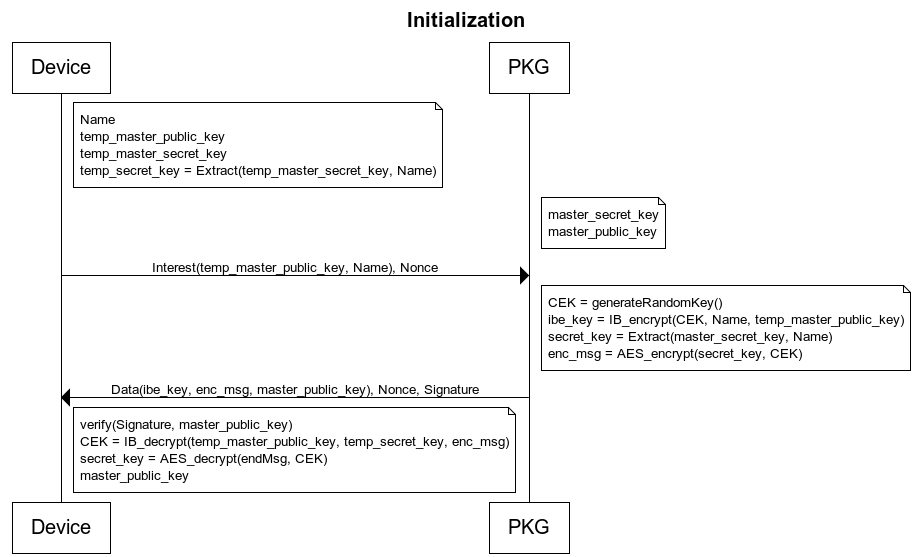
\includegraphics[width=1\textwidth]{Initialization.png}
%   \caption{Initialization IBE}
%   \label{fig:init_ibe_1}
% \end{figure}

Now that the mobile is authenticated, devices can connect to the mobile through e.g. \gls{NFC} for initialization.
This results in a rendezvous authentication between the device and the mobile, and if the mobile is given the authorities to perform initialization (\autoref{access_control}), the new device can join the \gls{PKG}s trust domain.

\subsubsection{Security Analysis}
It is important that the protocol possesses privacy, availability and control properties. 
I shortly present a formal security analysis by modeling the protocol in \gls{spdl} and verifying certain claims through Scyther~\cite{DBLP:conf/cav/Cremers08}.
After that, an informal discussion of the security in the protocol will be presented.

\textit{Scyther}.
The analysis proves that the protocol is confidential, replay and injection resistant, and possesses integrity and authenticity.
All claims made (i.e. \texttt{alive}, \texttt{secret}, \texttt{weakagree}, \texttt{niagree}, \texttt{nisynch}) shows no attacks in Scyther.
The \gls{spdl} code of the protocol can be reviewed in~\autoref{apx:scyther-analysis-dr}.

\textit{Authenticity}.
The protocol holds the required authenticity and integrity. 
The pre-shared temporary random key \texttt{tk} is shared in an assumed secure manner, thus appending an encrypted message to the Init Interest, is used as an authentication for the \gls{PKG}.
Thus the encryption, with the \texttt{tk} as key, protects against \gls{MITM} attacks.
The response \gls{data} is hashed and signed with the \gls{PKG}s \gls{SK} which provides authenticity and integrity for the requesting device.
The signature can easily be verified, and since an adversary do not obtain a polynomial time algorithm that can forge the \gls{SK} the device can be sure that the message is signed by the corresponding ID, which is the ID\textsubscript{PKG} received in the device registration phase 1, seen in~\autoref{fig:init_ibe_1}.
Thus the signature protects against \gls{MITM} attacks.

\textit{Confidentiality}. 
The \gls{SK} will be encrypted with the pre-shared temporary random key \texttt{tk}, and thus the confidentiality is preserved.
An adversary will only be able to know the \gls{MPK}, cipher texts, signatures and both IDs, which is not required to be confidential and not sufficient to compute the \gls{SK} that is extracted. 
The adversary do not obtain a polynomial time algorithm that can compute the \gls{SK} from the known parameters.
Hence an adversary have to obtain a algorithm to compute the secret keys, which is the same polynomial time algorithm as in the sub section above that the adversary do not have access to.

\textit{Replay}.
Since the adversary cannot compute \texttt{tk} nor forge the signature, it cannot send \gls{interest} nor \gls{data} that is captured at any arbitrary point. 
Devices keep track of the nonce corresponding to a data pull, hence a replay with will be detected and thrown away.

\subsection{Deployment Phase}\label{data_pull}
The goal for this protocol is to achieve a secure one-round data pull with authorization and integrity.
For the protocol to work and the data pull to be successful, 1) both devices has to belong to the same trust domain (i.e. has initialized with the same \gls{PKG}) and 2) the requester has to have granted access rights for the resource requested.

As illustrated in~\autoref{fig:health-sensor-system}, the device has joined the \gls{PKG}s trust domain and is ready to communicate with other devices.
This flow is illustrated in~\autoref{fig:data_pull_ibe}.
First the requester has to express an \gls{interest} to the target device asking for a specific resource. 
The \gls{receiver} checks whether the requester has access rights to the requested resource and verifies that the requester is a part of the same trust domain.
If the \gls{receiver} is authorized, the \gls{receiver} responds with the \gls{data} containing the resource. 
The requester signs the \gls{interest} and appends it to the content \gls{name}.
The \gls{receiver} will also do a symmetric encryption on the sensor \gls{data} and do a asymmetric encryption on the \gls{CEK} with the requester's \gls{ID}.
This step is only performed if \gls{data} confidentiality is needed. 
Then the \gls{data} packet is signed and sent.
Finally the requester receives the \gls{data}, verifies the signature and decrypts the sensor \gls{data}.

\begin{figure}[ht]
  \centering
  \begin{tikzpicture}[node distance=4.5cm,auto,>=stealth']
      \node[] (server) {PKG};
      \node[left = of server] (client_1) {Device};
      \node[left = of client_1] (client_0) {Mobile};
      \node[below of=server, node distance=8cm] (server_ground) {};
      \node[below of=client_0, node distance=8cm] (client_0_ground) {};
      \node[below of=client_1, node distance=8cm] (client_1_ground) {};
      %
      
      \draw (server) -- (server_ground);
      \draw (client_0) -- (client_0_ground);
      \draw (client_1) -- (client_1_ground);
      
      \draw ($(client_0)!0.10!(client_0_ground)$) 
      -- node[above,scale=0.8,right]{(ID\textsubscript{m}, sk\textsubscript{m}, mpk)} 
      ($(client_0)!0.10!(client_0_ground)$);
      \draw ($(client_1)!0.10!(client_1_ground)$) 
      -- node[above,scale=0.8,right]{(ID\textsubscript{d}, sk\textsubscript{d}, mpk)} 
      ($(client_1)!0.10!(client_1_ground)$);
      \draw ($(server)!0.10!(server_ground)$) 
      -- node[above,scale=0.8,left]{(msk, mpk)} 
      ($(server)!0.10!(server_ground)$);


      \draw ($(client_0)!0.15!(client_0_ground)$) 
      -- node[above,scale=0.8,right]{m\textsubscript{1} = (ID\textsubscript{d} || n || request)} 
      ($(client_0)!0.15!(client_0_ground)$);
      \draw ($(client_0)!0.20!(client_0_ground)$) 
      -- node[above,scale=0.8,right]{s\textsubscript{1} = Sign(mpk || sk\textsubscript{m} || c\textsubscript{1})} 
      ($(client_0)!0.20!(client_0_ground)$);
      \draw[->] ($(client_0)!0.35!(client_0_ground)$) 
      -- node[above,scale=0.8,midway]{Interest: m\textsubscript{1} || s\textsubscript{1}} 
      ($(client_1)!0.35!(client_1_ground)$);
      \draw ($(client_1)!0.40!(client_1_ground)$) 
      -- node[above,scale=0.8,right]{Verify(mpk || ID\textsubscript{m} || m\textsubscript{1} || sign)} 
      ($(client_1)!0.40!(client_1_ground)$);
      \draw ($(client_1)!0.45!(client_1_ground)$) 
      -- node[above,scale=0.8,right]{AccesControl(ID\textsubscript{m}, request)} 
      ($(client_1)!0.45!(client_1_ground)$);
      \draw ($(client_1)!0.50!(client_1_ground)$) 
      -- node[above,scale=0.8,right]{c\_cek = Encrypt(mpk || ID\textsubscript{d} || cek)} 
      ($(client_1)!0.50!(client_1_ground)$);
      \draw ($(client_1)!0.55!(client_1_ground)$) 
      -- node[above,scale=0.8,right]{c = AES\_Enc\textsubscript{cek}(data || \~{n})} 
      ($(client_1)!0.55!(client_1_ground)$);
      \draw ($(client_1)!0.60!(client_1_ground)$) 
      -- node[above,scale=0.8,right]{c\textsubscript{2} = (c\_cek || c)} 
      ($(client_1)!0.60!(client_1_ground)$);
      \draw ($(client_1)!0.65!(client_1_ground)$) 
      -- node[above,scale=0.8,right]{s\textsubscript{2} = Sign(mpk || sk\textsubscript{d} || c\textsubscript{2})} 
      ($(client_1)!0.65!(client_1_ground)$);
      \draw[<-] ($(client_0)!0.70!(client_0_ground)$) 
      -- node[above,scale=0.8,midway]{Data: c\textsubscript{2} || s\textsubscript{2}} 
      ($(client_1)!0.70!(client_1_ground)$);

      \draw ($(client_0)!0.80!(client_0_ground)$) 
      -- node[above,scale=0.8,right]{Verify(mpk || ID\textsubscript{d} || c\textsubscript{2} || sign)} 
      ($(client_0)!0.80!(client_0_ground)$);
      \draw ($(client_0)!0.85!(client_0_ground)$) 
      -- node[above,scale=0.8,right]{cek = Decrypt(mpk || ID\textsubscript{m} || c\_cek)}
      ($(client_0)!0.85!(client_0_ground)$);
      \draw ($(client_0)!0.90!(client_0_ground)$) 
      -- node[above,scale=0.8,right]{data, \^{n} = AES\_Dec\textsubscript{cek}(c)} 
      ($(client_0)!0.90!(client_0_ground)$);
      \draw ($(client_0)!0.95!(client_0_ground)$) 
      -- node[above,scale=0.8,right]{\^{n} == n} 
      ($(client_0)!0.95!(client_0_ground)$);
  \end{tikzpicture}
  \caption{Data pull under deployment. 
  The mobile sends a Sensor Interest to the device appending the request for a resource and a nonce \texttt{n}. 
  The Interest is signed with the mobile's secret key \texttt{sk\textsubscript{m}} and verified by the device. 
  The device checks whether the mobile has a valid capability for the requested resource and encrypts the data if granted.
  The Data response is signed with the device's secret key \texttt{sk\textsubscript{d}}.
  The mobile decrypts of the content encryption key \texttt{cek} and the cipher \texttt{c}, checks whether the received nonce \texttt{\^{n}} is equal to \texttt{n} and finally accepts the data as correct.}
  \label{fig:data_pull_ibe}
\end{figure}

% \begin{figure}[ht]
%   \centering
%   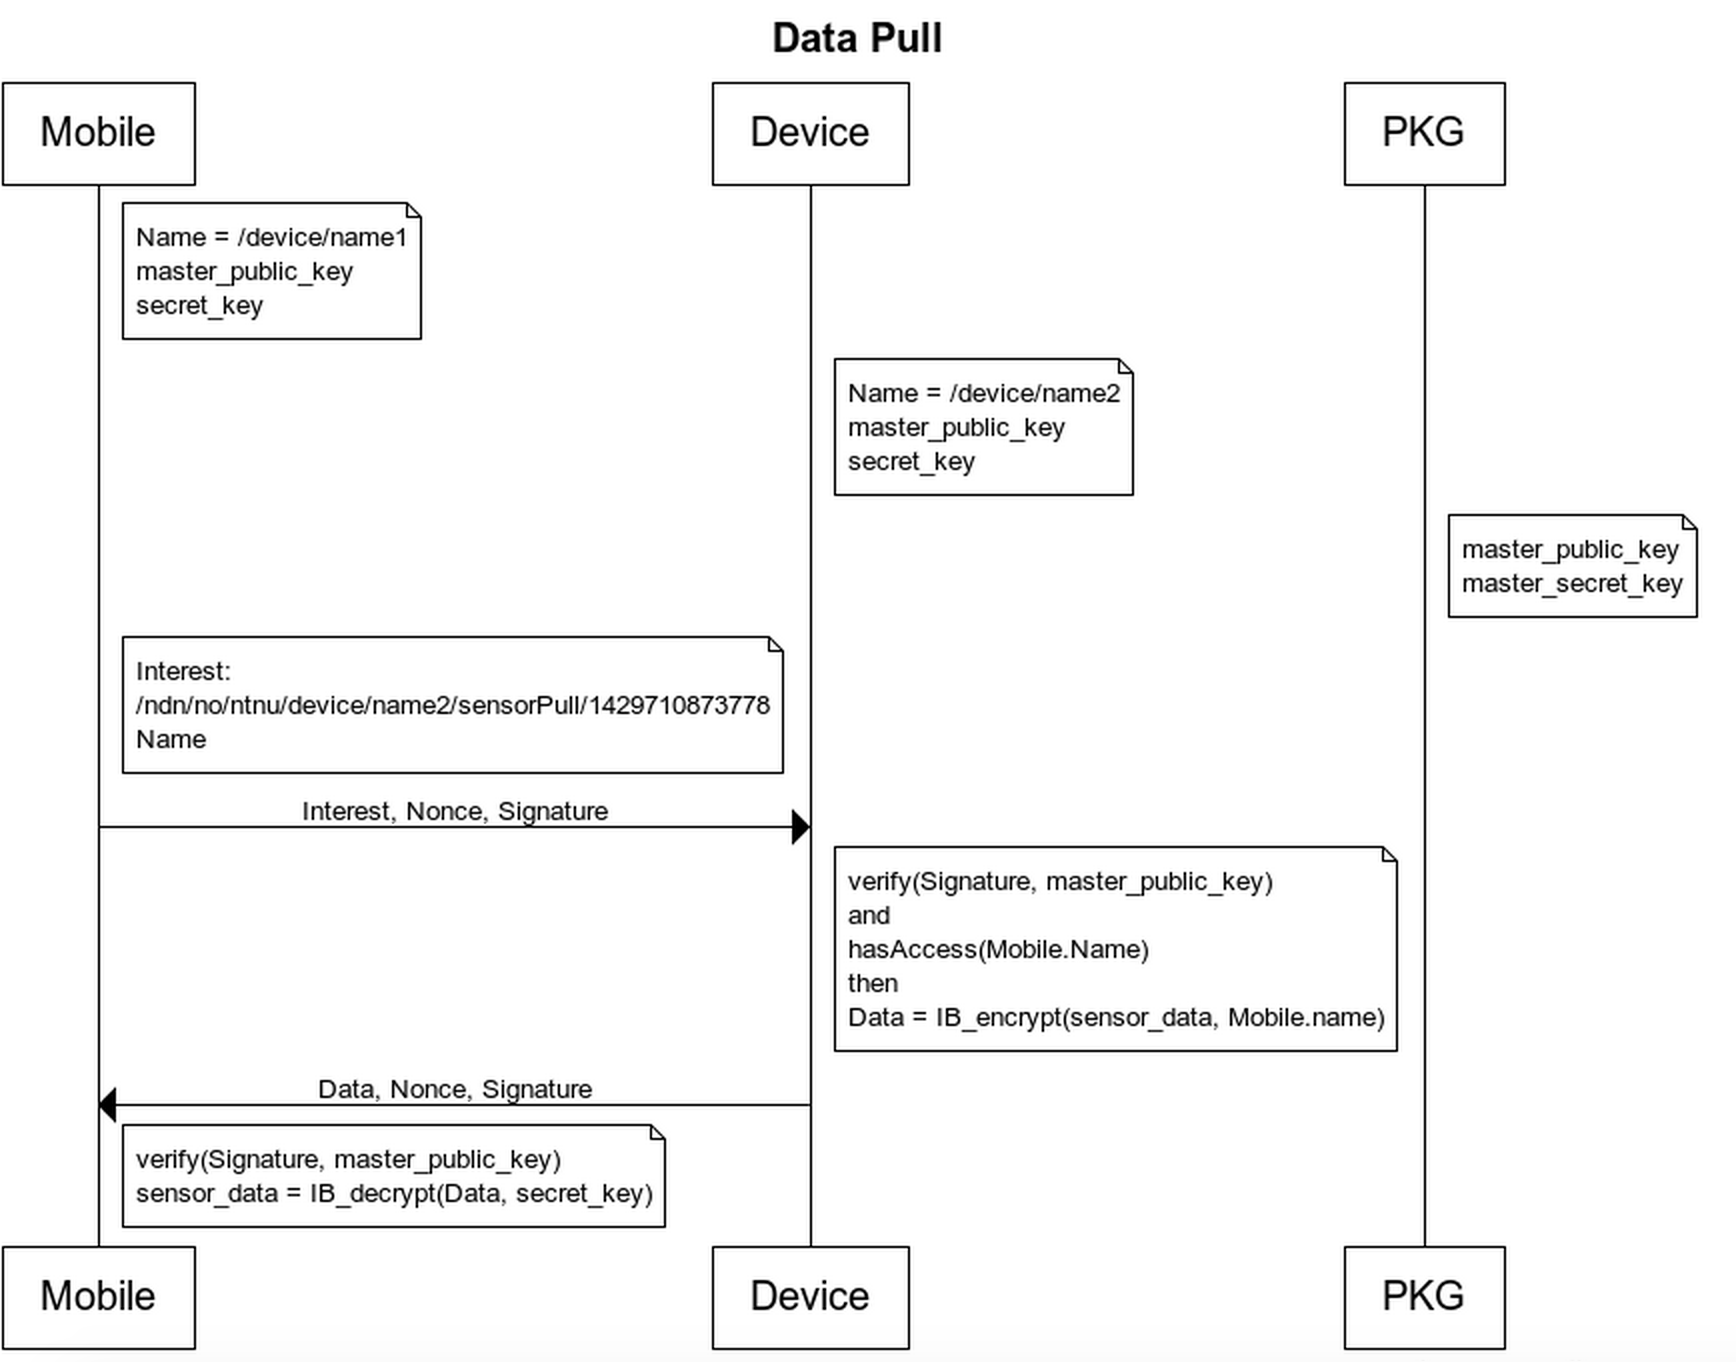
\includegraphics[width=1\textwidth]{DataPull.png}
%   \caption{Mobile performing a data pull from a device in the network.}
%   \label{fig:data_pull_ibe}
% \end{figure}

\subsubsection{Security Analysis}
It is important that the protocol possesses privacy, availability and control properties. 
I shortly present a formal security analysis by modeling the protocol in \gls{spdl} and verifying certain claims through Scyther.
After that, an informal discussion of the security in the protocol will be presented.

\textit{Scyther}.
The analysis proves that the protocol is confidential, replay and injection resistant, and possesses integrity and authenticity.
All claims made (i.e. \texttt{alive}, \texttt{secret}, \texttt{weakagree}, \texttt{niagree}, \texttt{nisynch}) shows no attacks in Scyther. 
The \gls{spdl} code of the protocol can be reviewed in~\autoref{apx:scyther-analysis-dp}.

\textit{Authenticity}.
The protocol holds the required authenticity and integrity. 
The message is hashed and signed with the senders \gls{SK} which provides authenticity and integrity.
The signature can easily be verified by the receiver, and since an adversary do not obtain a polynomial time algorithm that can forge the \gls{SK} one can be sure that the message is signed by the corresponding ID.
Thus the signature protects against \gls{MITM} attacks.

\textit{Confidentiality}. 
All \gls{data} that flows through the \gls{HSS} can be encrypted if necessary. 
When a resource is requested, the \gls{publisher} will do an access control to decide whether the ID\textsubscript{requester} has the right capabilities. 
The \gls{CEK} will be asymmetrically encrypted, and the resource data will be symmetrically encrypted, thus both key and data is confidential and only available to whoever has the corresponding \gls{SK} to the ID\textsubscript{requester}.
An adversary will only be able to know the \gls{MPK}, nonce, request, cipher and both IDs, which is not required to be confidential and not sufficient to compute the resource data. 
The adversary do not obtain a polynomial time algorithm that can compute the resource data from the known parameters.
Hence an adversary have to obtain a algorithm to compute the secret keys, which is the same polynomial time algorithm as in the sub section above that the adversary do not have access to.

\textit{Replay}.
Since the adversary cannot forge the signature, it cannot send \gls{interest} nor \gls{data} that is captured at any arbitrary point. 
This is due to the nonce presence in all packets. 
Devices keep track of the nonce corresponding to a data pull, hence a replay with will be detected and thrown away.

\subsection{Key Distribution using File Synchronization Module}

The Stig wants to have full control over the devices that are a part of the trust domain, and be able to remove a device if necessary.
Each device should have an updated list of all public keys, i.e. every devices' \gls{ID}.
The \gls{ID} of every device is a part of the \gls{name}.
A device register the prefix \path{/ndn/no/ntnu/<device>/<resource>} and hence its \gls{ID} is \path{/ndn/no/ntnu/<device>}.
The distribution of this list can easily be achieved by using the \gls{FSM} (\autoref{file-sync} \& \autoref{key-distribution}).
The \gls{PKG} will be the distributor in this synchronization and each device will be a subscriber.


\section{Security Analysis}
\todo{refactor section}
In this section the security of the protocols presented in~\autoref{init} and ~\autoref{data_pull} will be proven.

\subsection{Threat Model}
Threats that I find relevant for the \gls{HSS} can be categorized into three main categories: threats to privacy, threats to availability and threats to control.
I assume the following threat model:
\begin{enumerate}
  \item An adversary might try to eavesdrop information (privacy).
  \item An adversary might try to send bogus commands, e.g. injection, replay and \gls{MITM} (control).
  \item Jamming, node compromise (such as theft of mobile) and \gls{DoS} (availability).
\end{enumerate}

I assume that the \gls{PKG} cannot be compromised by any adversary, and thus the \gls{MSK} will always be hidden from any adversaries. 
However, it is extremely important that the machine which plays the role of the \gls{PKG} is secured in a physical matter, as well as remote secureness. 
The \gls{PKG} is the single point of failure in the whole system.

An idea introduced by Aaditeshwar Seth and Srinivasan Keshav in~\cite[Section 5.4]{Seth:2005:PSD:1897159.1897165} is to avoid storing the \gls{SK}s in devices that is more likely to be lost or stolen, e.g. a mobile.
Using \gls{HIBC}, one can extend the key hierarchy by another level that is time-based.
These time-based keys can then be downloaded to the mobile on a daily basis, hence the time the mobile will be compromised is reduced.

\subsection{Access Control}\label{access_control}
Since the ID\textsubscript{device} is appended to the \gls{interest} and the \gls{interest} is signed by the corresponding SK\textsubscript{device}, the \gls{ID} of the device can easily be authenticated. 
When a device retrieves an \gls{interest} for its sensor \gls{data}, there should be an authorization mechanism. 
One can argue that once a device has been authenticated in the \gls{PKG}s trust domain, everyone in the domain can be sure that the device will not abuse the information or functionalities available. 
However, due to scalability this is not a secure way to handle access control. 
If a device does not need a privilege, it does not need it.
Hence it should not have it. 
That is the least privilege access principle, which is default in Capability Based Approach to \gls{IoT} Access Control~\cite{DBLP:conf/imis/GusmeroliPR12}.
This approach has some additional benefits for the \gls{HSS}, such as

\begin{itemize}
  \item delegation support - 
  A device can grant access rights to other devices, as well as granting the right to further delegate these rights to a third device.
  \item capability revocation - 
  If the \gls{PKG} have granted delegation rights to a mobile, and the mobile is not found trustworthy after a while, the capabilities issued by the mobile can easily be revoked.
  \item information granularity - 
  Specific resources from a device can be granted access to in different granularity.
\end{itemize}

Another solution can be an \gls{ACL} based approach equivalent to what Wentao Shang et al. did in~\cite{DBLP:journals/network/ShangDMBZ14}.

\subsection{Confidentiality}
The confidentiality is achieved by doing asymmetric encryption on a \gls{CEK} that is used for symmetric encryption on the content.
As explained in the sequence diagram (\autoref{fig:data_pull_ibe}) presented in the above sections, each \gls{interest} appends the requester's ID (\autoref{eq:mapping-id-name-pk}).
Since the ID\textsubscript{requester} always is appended it can always be used to do asymmetric encryption, hence all \gls{CEK}s can be encrypted only for the requesting device, and thus the confidentiality in the system can always be achieved.

\subsection{Integrity and Authenticity}
Each device will obtain a secret key allocated by its superior \gls{PKG}, as explained in~\autoref{ibc}.
With the concept from~\autoref{rendezvous_authentication} together with the \gls{PKG}s \gls{MPK}, you can trust that the device is authorized for the \gls{PKG}s trust domain. 
Hence all signed packets can be verified by anyone with the \gls{MPK}.
In this setting, a verified signature acts as an assurance of authentication and integrity. 

Every \gls{interest} has a timestamp attached to the \gls{name} (e.g. \path{/ndn/no/ntnu/device/name2/sensorPull/1429710873778}), i.e. milliseconds from \texttt{UTC} \texttt{1970-01-01} \texttt{00:00:00}, that can be used for protection against replay attack. 

\subsection{Availability}
This is a harder problem to solve.
The network is purely wireless, hence vulnerable to jamming. 
An adversary could try to send infinite \gls{interest}s to a device with an invalid signature, hence the device may be overloaded with work and might run out of battery fast.
Therefore one should check the \gls{MPK} before doing any crypto.
This is also why I have chosen to append the MPK in the packet~\autoref{fig:sensor_interest-data}. 

\subsection{Trust Model}
For a system to be secure, cryptography together with trust is essential. 
The \gls{HSS} trust model is built upon trusting a centralized authority, typically the user's home server, rendezvous authentication and \gls{IBC}.
The fact that it runs over \gls{NDN} makes it easier to achieve security goals and usability for third party developers.

The \gls{PK} is the \gls{name} of the device, and all content published by the device will begin with this \gls{name}, hence it is easy to verify that the \gls{publisher} is the owner of the content.
To be able to verify and encrypt messages, the device need the MPK\textsubscript{PKG} and the ID of the user it wants to communicate with. 
If allowed by the PKG, the public parameters MPK\textsubscript{PKG} is public for everybody that is not a part of the trust domain. 
To be able to sign and decrypt messages the device have to be a member of the trust domain and be issued a secret key mapping to the ID\textsubscript{device}.
Each device builds its trust on other devices based on that it has been verified by an administrator that controls the \gls{PKG}.
